\documentclass[tikz,border=10pt]{standalone}
\usepackage[T1]{fontenc}
\usepackage{lmodern}
\usetikzlibrary{arrows.meta, positioning, fit}

\definecolor{ink}{HTML}{334155}
\definecolor{inputbg}{HTML}{F8FAFC}
\definecolor{sharedbg}{HTML}{EFF6FF}
\definecolor{actorbg}{HTML}{EEF2FF}
\definecolor{criticbg}{HTML}{ECFDF5}
\definecolor{pointerbg}{HTML}{FFF7ED}
\definecolor{outputbg}{HTML}{FEFCE8}

\tikzset{
  box/.style={
    draw=ink,
    rounded corners=5pt,
    line width=0.8pt,
    align=left,
    inner sep=7pt,
    font=\sffamily\small
  },
  input/.style={box, fill=inputbg, text width=55mm},
  process/.style={box, fill=sharedbg, align=center, text width=43mm},
  actor/.style={box, fill=actorbg, align=center, text width=47mm},
  critic/.style={box, fill=criticbg, align=center, text width=47mm},
  pointer/.style={box, fill=pointerbg, text width=55mm},
  output/.style={box, fill=outputbg, align=center, minimum width=31mm},
  note/.style={box, fill=inputbg, text width=49mm, font=\sffamily\footnotesize},
  arrow/.style={-{Latex[length=2.5mm]}, line width=0.8pt, draw=ink}
}

\begin{document}
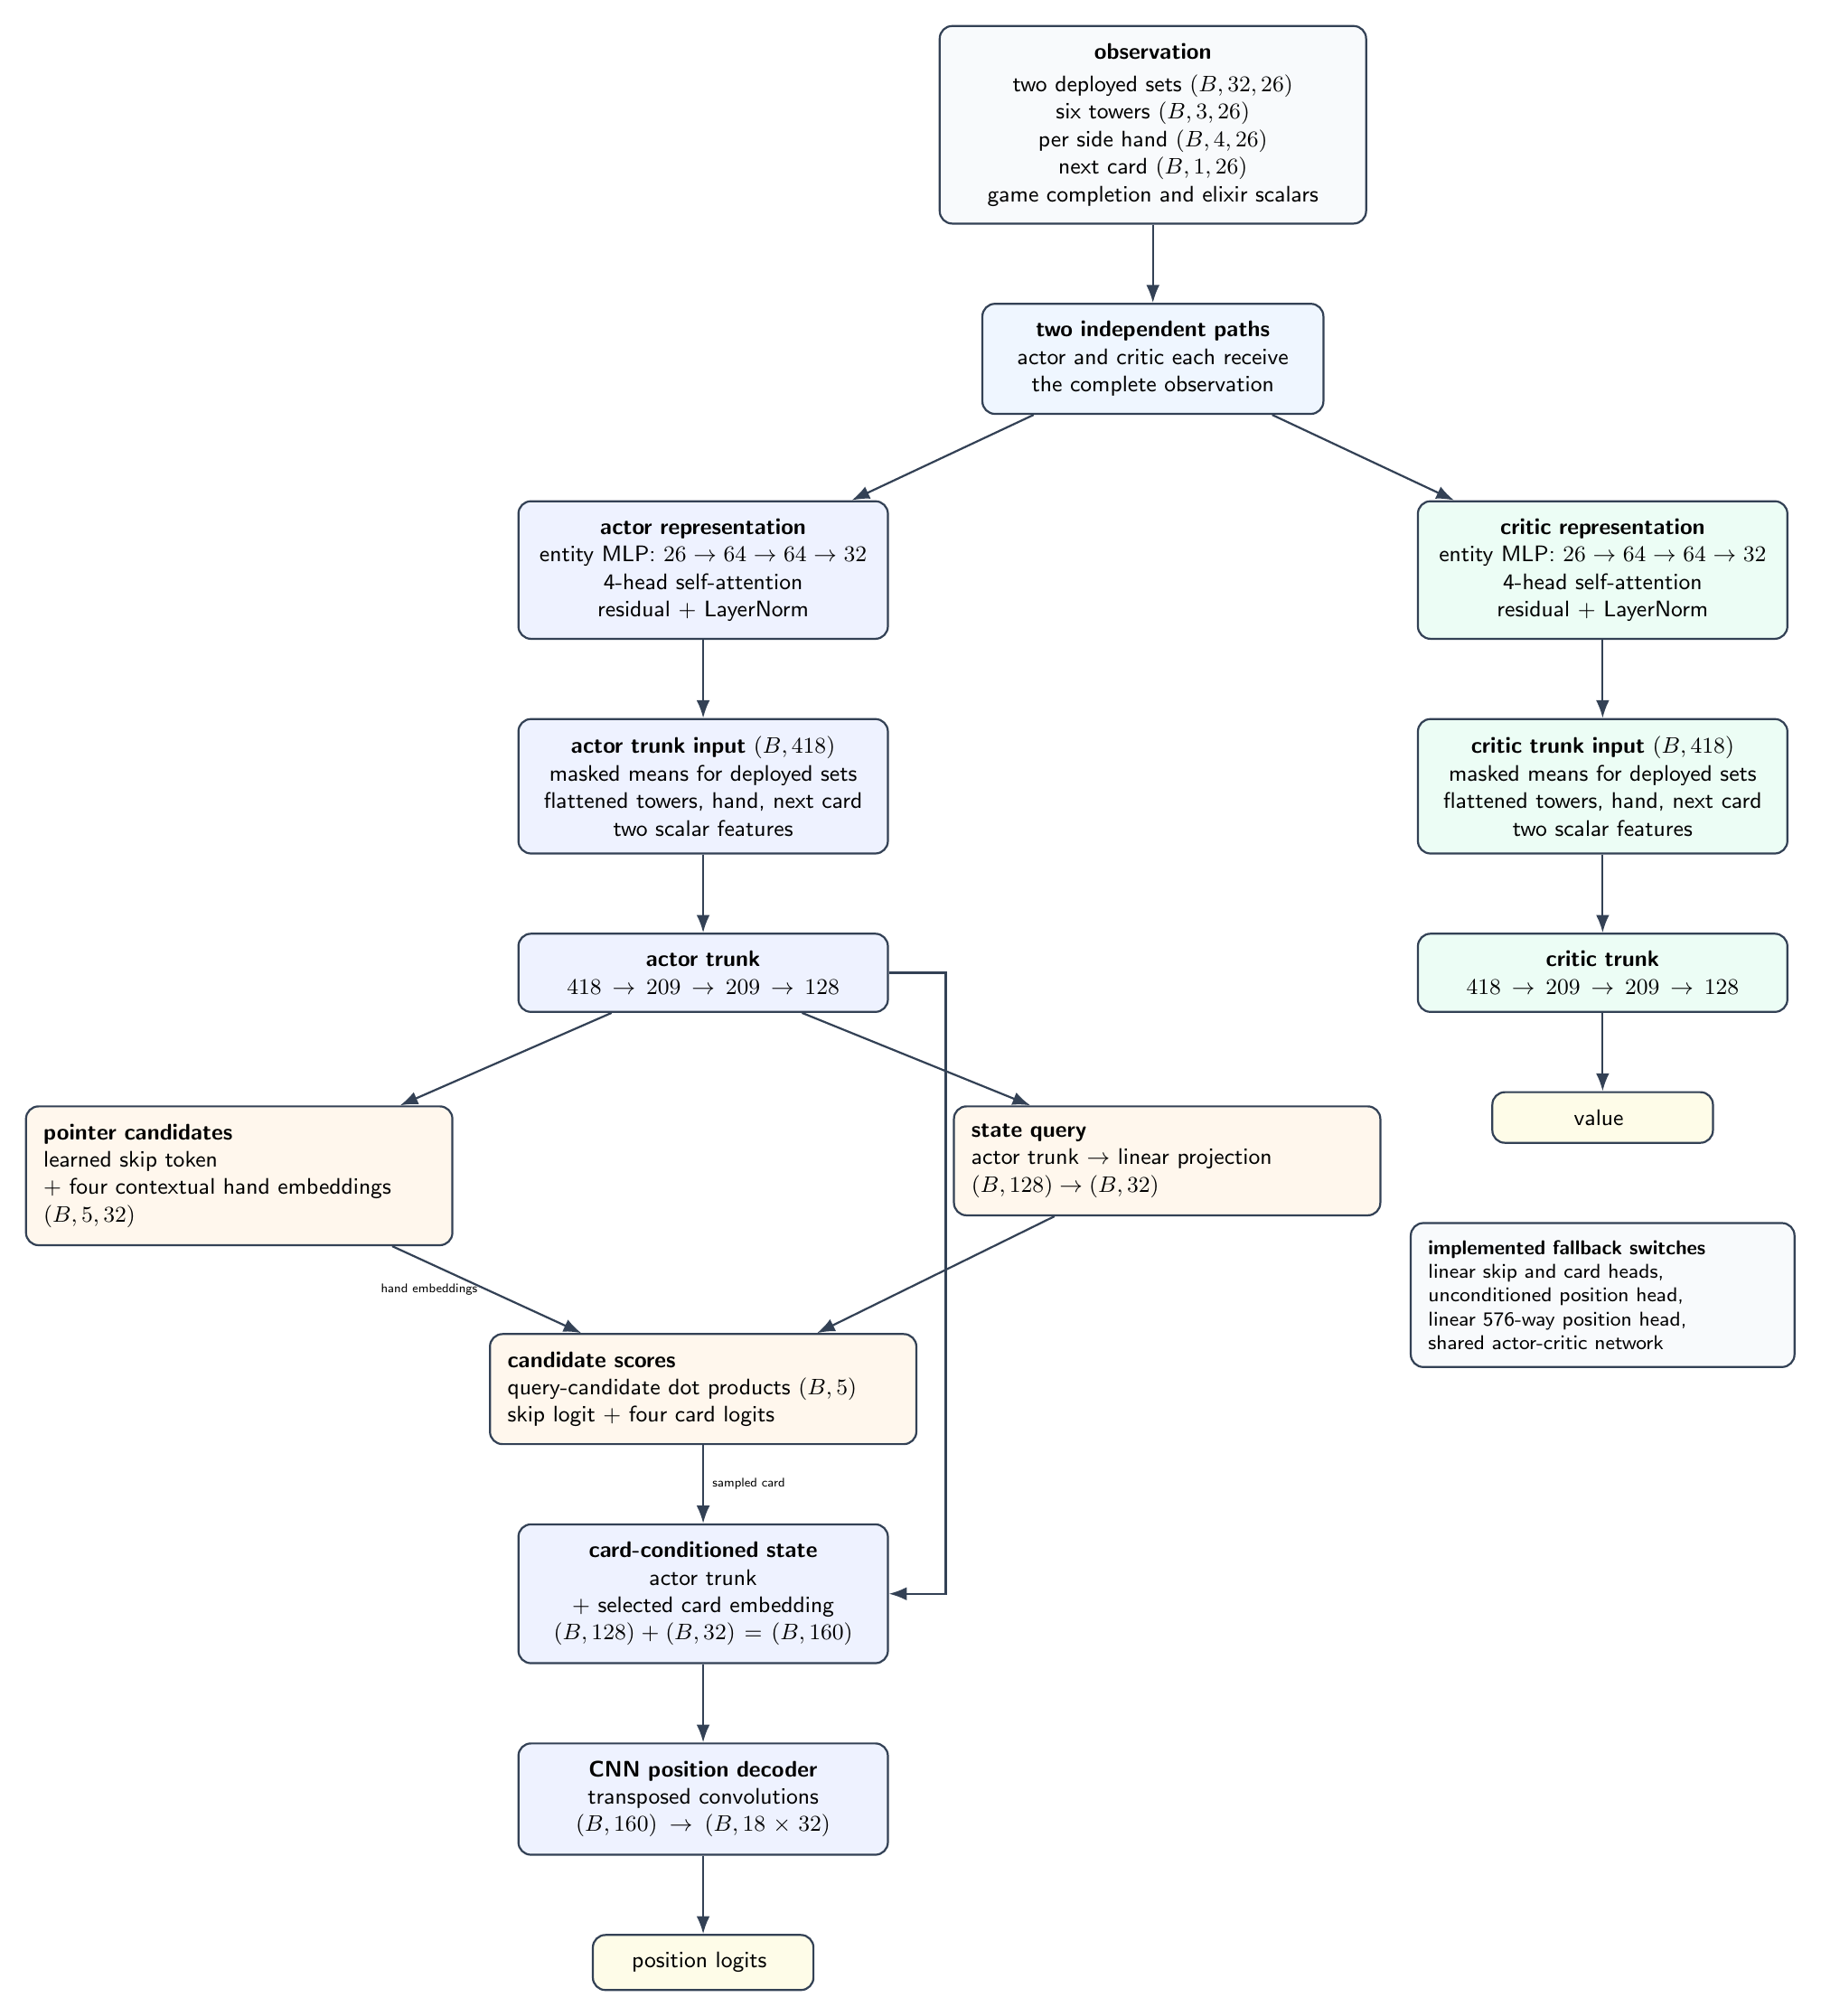
\begin{tikzpicture}[node distance=11mm and 15mm]

\node[input, align=center] (obs) {
  \textbf{observation}\\[2pt]
  two deployed sets $(B,32,26)$\\
  six towers $(B,3,26)$\\
  per side hand $(B,4,26)$\\
  next card $(B,1,26)$\\
  game completion and elixir scalars
};

\node[process, below=of obs] (split) {
  \textbf{two independent paths}\\
  actor and critic each receive\\
  the complete observation
};

\node[actor, below left=12mm and 13mm of split] (actorenc) {
  \textbf{actor representation}\\
  entity MLP: $26\to64\to64\to32$\\
  4-head self-attention\\
  residual + LayerNorm
};

\node[critic, below right=12mm and 13mm of split] (criticenc) {
  \textbf{critic representation}\\
  entity MLP: $26\to64\to64\to32$\\
  4-head self-attention\\
  residual + LayerNorm
};

\node[actor, below=of actorenc] (actorpool) {
  \textbf{actor trunk input $(B,418)$}\\
  masked means for deployed sets\\
  flattened towers, hand, next card\\
  two scalar features
};

\node[critic, below=of criticenc] (criticpool) {
  \textbf{critic trunk input $(B,418)$}\\
  masked means for deployed sets\\
  flattened towers, hand, next card\\
  two scalar features
};

\node[actor, below=of actorpool] (actortrunk) {
  \textbf{actor trunk}\\
  $418\to209\to209\to128$
};

\node[critic, below=of criticpool] (critictrunk) {
  \textbf{critic trunk}\\
  $418\to209\to209\to128$
};

\node[output, below=of critictrunk] (value) {
  value
};

\node[pointer, below left=13mm and 9mm of actortrunk] (candidates) {
  \textbf{pointer candidates}\\
  learned skip token\\
  + four contextual hand embeddings $(B,5,32)$
};

\node[pointer, below right=13mm and 9mm of actortrunk] (query) {
  \textbf{state query}\\
  actor trunk $\to$ linear projection\\
  $(B,128)\to(B,32)$
};

\node[pointer, below=45mm of actortrunk] (scores) {
  \textbf{candidate scores}\\
  query-candidate dot products $(B,5)$\\
  skip logit + four card logits
};

\node[actor, below=of scores] (condition) {
  \textbf{card-conditioned state}\\
  actor trunk\\
  + selected card embedding\\
  $(B,128)+(B,32)=(B,160)$
};

\node[actor, below=of condition] (cnn) {
  \textbf{CNN position decoder}\\
  transposed convolutions\\
  $(B,160)\to(B,18\times32)$
};

\node[output, below=of cnn] (position) {
  position logits
};

\node[note, below=of value] (fallback) {
  \textbf{implemented fallback switches}\\
  linear skip and card heads,\\
  unconditioned position head,\\
  linear 576-way position head,\\
  shared actor-critic network
};

\draw[arrow] (obs) -- (split);
\draw[arrow] (split) -- (actorenc);
\draw[arrow] (split) -- (criticenc);
\draw[arrow] (actorenc) -- (actorpool);
\draw[arrow] (criticenc) -- (criticpool);
\draw[arrow] (actorpool) -- (actortrunk);
\draw[arrow] (criticpool) -- (critictrunk);
\draw[arrow] (critictrunk) -- (value);
\draw[arrow] (actortrunk) -- (query);
\draw[arrow] (actortrunk) -- (candidates);
\draw[arrow] (query) -- (scores);
\draw[arrow] (candidates) -- node[left, font=\sffamily\tiny] {hand embeddings} (scores);
\draw[arrow] (actortrunk.east) -- ++(8mm,0) |- (condition.east);
\draw[arrow] (scores) -- node[right, font=\sffamily\tiny] {sampled card} (condition);
\draw[arrow] (condition) -- (cnn);
\draw[arrow] (cnn) -- (position);

\end{tikzpicture}
\end{document}
